\chapter{A New Cosmology\label{chap_ANC}}
\epigraph{We have introduced a new and far-reaching principle into the relativity theory, viz.~that symmetry itself can only be relative; and the particle, which so far as mechanics is concerned is to be identified with its gravitational field, is the standard of symmetry.}{---Sir Arthur Stanley~Eddington, \textit{The Mathematical Theory of Relativity}}
\section{Global Parametrisation of Spacetime in a Massive Rest-Frame\label{sec_GPSMRF}}
According to the discussion in Chapter~\ref{chap_DIRT}, we shall proceed here with the analysis of a comoving 3-sphere which expands from a finite minimum radius that is well-defined in its subsisting de~Sitter void, based on the additional prior physical assumption, that the cosmic rest-frame of massive particles \textit{is} the collection of null-lines emanating in one direction through that void, with `massless' photons defined as the particles which move at the same rate relative to this fundamental rest-frame---i.e., either zero velocity through the actual universe, or twice that of a null line,---so that the spacetime paths of massive particles and photons may be described by defining photon geodesics as null rays in the line-element corresponding to the perception of events in that frame, given by Eq.~(\ref{sphersymm_r}).\footnote{In this chapter, we will drop the subscript from $r_{\mathrm{SdS}}$ and $t_{\mathrm{SdS}}$, which are the primary such coordinates analysed here. They are not to be confused with the $r$ and $t$ coordinates defined in Eqs.~(\ref{max_symm}) and (\ref{r(t)}).} And the analysis in this chapter will eventually justify the subsequent assertion that was made there, that such a universe would actually appear to all observers, if they would model the universe's large-scale evolution using the proper line-element in the cosmic rest-frame, precisely as a flat $\Lambda$CDM universe that began from a singularity at the beginning of cosmic time. 

In order to justify that assertion, however, it is not enough to consider only the model that would be used to describe the observed cosmic expansion rate, but we must also work out what the large-scale structure of all matter in the universe should be, and how it would appear to massive observers. We will come to that description through a determination of the physical parametrisation of the spacetime geometry which applies not only to the cosmic rest-frame, but similarly to the geometry that describes any local massive frame which may be considered on a large enough scale that overall charge and spin should be negligible, which might instead be given by the alternate form of the metric, Eq.~(\ref{sphersymm_t}). After the physical parametrisation of the geometries and the cosmographical theory have been completed in this section and the next, we will proceed, in \S~\ref{sec_MC}, to determine the line-element in the proper time coordinate system of the fundamental rest-frame, and the corresponding cosmological model. Finally, in \S~\ref{sec_CBHO}, we shall conclude with the qualitative description of a scenario for the birth of such a universe following from gravitational collapse in a similar prior one.

Thus, we begin by determining possible restrictions on the coefficients $A(r,t)$ and $B(r,t)$ in Eq.~(\ref{sphersymm_r}), when the metric tensor is required to satisfy the field equation, $R_{\mu\nu}=\Lambda{g}_{\mu\nu}$; in particular, we immediately note that
\begin{equation}
0=R_{rt}=R_{tr}=-\frac{1}{rB(r,t)}\frac{\partial{B(r,t)}}{\partial{t}}.\label{R_rt}
\end{equation} 
Therefore, $B(r,t)$ must be a function of $r$ only, which we make use of in order to simplify the expressions for the remaining components of the Ricci tensor ($X'\equiv\partial{X}/\partial{r}$):
\begin{eqnarray}
R_{rr}\!\!\!&=&\!\!\!-\frac{B}{4A'}\frac{\partial}{\partial{r}}\left(\frac{{A'}^2}{AB}\right)+\frac{B'}{Br},\label{R_rr}\\
R_{tt}\!\!\!&=&\!\!\!\frac{A}{4A'}\frac{\partial}{\partial{r}}\left(\frac{{A'}^2}{AB}\right)+\frac{A'}{Br},\label{R_tt}\\
R_{\theta\theta}\!\!\!&=&\!\!\!1+\frac{1}{B}-\frac{B'r}{2B^2}+\frac{A'r}{2AB},\label{R_thetatheta}\\
R_{\phi\phi}\!\!\!&=&\!\!\!{R_{\theta\theta}}\sin^2\theta; \label{R_{phiphi}}
\end{eqnarray}
so that, according to the vacuum Einstein equation, we may write,
\begin{equation}
\frac{R_{rr}}{B}+\frac{R_{tt}}{A}=\frac{(AB)'}{AB^2r}=0.
\end{equation}

Therefore, $(AB)'=0$, and we may generally write $A(r,t)=f(t)/B(r)$; but then $f(t)$ may be gauged away by re-defining $t$ through $dt\mapsto{dt'}=\sqrt{f(t)}dt$, so that
\begin{equation}
A(r)=\frac{1}{B(r)}\label{AB(r)},
\end{equation} 
which generalises the Jebsen-Birkhoff theorem \cite{Jebsen1921,Jebsen2005,Birkhoff1923} to non-zero $\Lambda$, as proven by Lema\^{i}tre in 1931 \cite{Lemaitre1931b}, according to which the metric of spherically symmetric spacetime beyond a non-charged mass may always be written with an additional $t$-like Killing vector field. For a more detailed analysis, see \cite{Schleich2010}, which generalises the statement of the theorem and its proof to include the Nariai solution \cite{Nariai1950,Nariai1999a,Nariai1951,Nariai1999b}, 
\begin{equation}
ds^2=-\left(1-\Lambda{r^2}\right)dt^2+\frac{dr^2}{1-\Lambda{r^2}}+\frac{1}{\Lambda}\left(d\theta^2+\sin^2\theta{d\phi^2}\right).\label{Nariai}
\end{equation}

Now, we also have the requirement that $R_{\theta\theta}=\Lambda{r^2}$; thus, insertion of Eq.~(\ref{AB(r)}) into Eq.~(\ref{R_thetatheta}) yields
\begin{equation}
1+\frac{1}{B}-\frac{B'r}{B^2}=1+\frac{d}{dr}\left(\frac{r}{B}\right)=\Lambda{r^2},\label{diff_B}
\end{equation}
or
\begin{equation}
1+A+A'r=1+\frac{d}{dr}\left(Ar\right)=\Lambda{r^2};\label{diff_A}
\end{equation}
either of which may be directly integrated, with the result,
\begin{equation}
A(r)=\frac{1}{B(r)}=\frac{\frac{\Lambda}{3}r^3-r-\left(\frac{\Lambda}{3}{r_0}^3-r_0\right)+A(r_0)r_0}{r},\label{A(r)}
\end{equation}
where $r_0$ is some limit of the coordinate $r$. 

So far, no constraint has been given on $r$, other than the requirement of its definition, that hyper-surfaces of constant $r$ and $t$ will have an area $4\pi{r^2}$, which defines it as `the radius', and allows us to set $g_{\theta\theta}\equiv{r^2}$. In fact, this does not even require $r$ to be positive. In order to make this definition, however, $r=0$ needs to be relinquished as a coordinate singularity of the metric. Actually, when the integration constant in Eq.~(\ref{A(r)}),
\begin{equation}
2M\equiv{r_0-\frac{\Lambda}{3}{r_0}^3+A(r_0)r_0},\label{2M}
\end{equation}
is not zero, $r=0$ is the well-known black hole singularity (cf.~Eq.~(\ref{SdS_statical})). Integration of Eqs.~(\ref{diff_B}) and (\ref{diff_A}) is therefore not valid across this value.

Furthermore, we should observe that $r_0$ is a horizon of the geometry if, and only if, $A(r_0)=1/B(r_0)=0$. Then, it is a coordinate singularity through which we also may not integrate, and, as such, an appropriate reference point from which to parametrise the solution; we therefore set $A(r_0)\equiv0$, in order to provide physical meaning to the other integration constant, $r_0$. 

But also, since $\Lambda>0$ by definition on our underlying void, it is extremely useful to write the solution in a scale-invariant form, normalising all dimensional quantities with the universal `quadric of curvature', as Eddington called it, according to $s\mapsto{s'}=\sqrt{\Lambda/3}s$, $t\mapsto{t'}=\sqrt{\Lambda/3}t$, $r\mapsto{r'}=\sqrt{\Lambda/3}r$, and $r_0\mapsto{{r_0}'}=\sqrt{\Lambda/3}r_0$ ($\Rightarrow{M}\mapsto{M'}=\sqrt{\Lambda/3}M$), so that the metric can finally be written,
\begin{equation}
ds^2=-\frac{r}{r^3-{r_0}^3-(r-r_0)}dr^2+\frac{r^3-{r_0}^3-(r-r_0)}{r}dt^2+r^2(d\theta^2+\sin^2\theta{d\phi^2}).\label{SdS_statical_pure}
\end{equation}

Obviously, this solution always has the one horizon, at $r=r_0$, as our definition of $r_0$ requires; but when ${r_0}^2\leq4/3$ there are actually two more, at $r=-\frac{r_0}{2}\pm\frac{1}{2}\sqrt{-3r_0^2+4}$;---i.e., when this condition is met, there are three real solutions to the horizon equation, 
\begin{equation}
r^3-{r_0}^3-(r-r_0)=0,\label{horizon_eq}
\end{equation}
and the two horizons that exist in addition to the one which is always explicitly defined at $r=r_0$, are on the ellipse, \begin{equation}
r^2+rr_0+{r_0}^2=1.\label{SdS_ellipse}
\end{equation} 

When ${r_0}^2<4/3$ \textit{and} ${r_0}^2\neq1/3$ (i.e., $M^2<1/27$), and the line-element has three distinct singularities in addition to the one at $r=0$, positive $r$ is spacelike on some interval, and the solution is in the form given by Eq.~(\ref{sphersymm_t}), with $C(r,t)\equiv{r^2}$, which describes spacetime surrounding an uncharged, non-spinning mass, in which radial photons move isotropically along null-lines. This shall be referred to as the \textit{under-critical} SdS geometry.

When the condition, $r_0^2=4/3$ or 1/3 $(M^2=1/27)$, for the \textit{critical} SdS geometry is met, there are precisely two horizons: one at $r=r_0$, and another at $r=-r_0/2$ or $-2r_0$, as the case may be---i.e., the two horizons of the two critical SdS geometries are at ${r}=\pm2/\sqrt{3}$ and $\mp1/\sqrt{3}$, with corresponding mass parameter, $M=\mp1/\sqrt{27}$.

And when ${r_0}^2>4/3$ $(M^2>1/27)$, there is only one real root of Eq.~(\ref{horizon_eq}), and the sign of $M$ differs from that of $r_0$. The line-element of this \textit{over-critical} SdS geometry, which is timelike for all $r>0$ when $M>1/\sqrt{27}$ $(r_0<-2/\sqrt{3})$, provides an ideal spacetime description of our universe, which begins from an initial singularity at $r=0$, and expands as the cosmic time, $r$, increases. But $r=0$ is very different from the \textit{big bang} singularities of the dynamical FLRW universes which must emerge in some manner like the Einstein-de~Sitter universe, so that, as Eddington put it, `in the beginning all the matter created was projected with a radial motion so as to disperse even faster than the present rate of dispersal of galaxies' \cite{Eddington1933}---for this property is common to the initial states of all such universes, since the description at the beginning is not essentially different even if some `dark energy'---even a quintessence field that could be linked to the inflation scenario---should eventually take over as the dominant cause of expansion. Instead, the SdS singularity at $r=0$ is of the de~Sitter-type, and therefore much like that of the Lema\^{i}tre-Robertson universe, about which Weyl wrote, `If I think about how, on the de~Sitter hyperboloid the world lines of a star system with a common asymptote rise up from the infinite past, then I would like to say: the World is born from the eternal repose of `Father {\AE}ther'; but once disturbed by the `Spirit of Unrest' (\textit{H\"{o}lderlin}), which is at home in the Agent of Matter, `in the breast of the Earth and Man', it will never come again to rest' \cite{Weyl1924}; so the mathematical description of cosmic expansion is in fact consistent with Eddington's interpretation.

\begin{figure}[t!]
\centerline{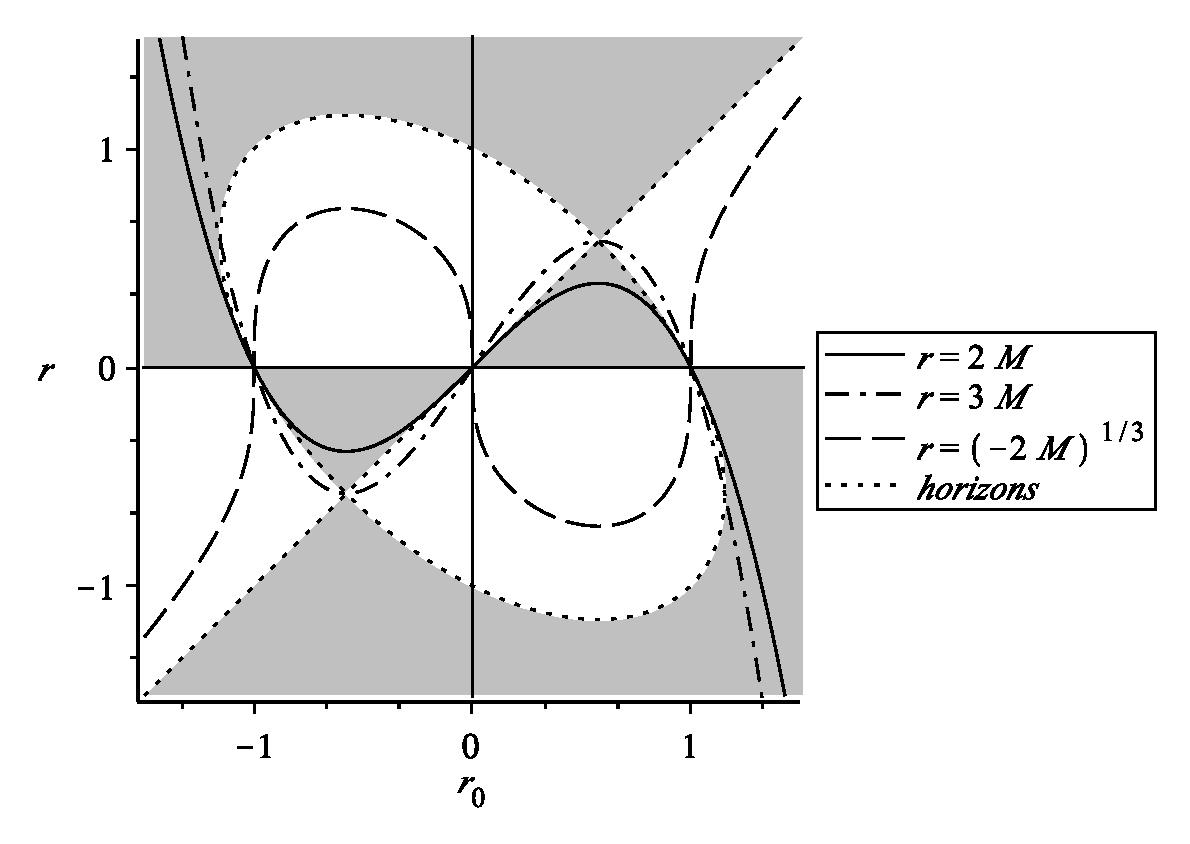
\includegraphics[width=6.5in]{fund_ellipse.eps}}
\caption[Scale-invariant horizons of the SdS geometries.]{A scale-invariant picture of the SdS geometries in the $(r,r_0)$-plane, with various interesting values of $r$ plotted as functions of $r_0$. In shaded and unshaded regions, $g_{rr}<0$ and $g_{rr}>0$, respectively.}\label{SdS_scaleinv}
\end{figure}
The global parametrisation of the SdS geometries is graphed in Fig.~\ref{SdS_scaleinv}. In the shaded regions $r$ is `timelike', and in the unshaded regions it is `spacelike'. The radius at which the gravitational potential vanishes identically, $r=\sqrt[3]{-2M}\equiv\sqrt[3]{{r_0}^3-r_0}$, has been plotted along with two other radii of interest, $r=2M$ and $r=3M$. It is important to note, that the geometry for any particular value of $r_0$, when ${r_0}^2\leq4/3$, is precisely the same as when $r_0$ has instead the value of either of the other two horizon radii, as it must be, according to the explicit definition of the cubic \textit{mass parameter}, $M$. In other words, the geometries in the parametric range, $-2/\sqrt{3}\leq{r_0}\leq-1$, are formally equivalent to those in the intervals, $0\leq{r_0}\leq1/\sqrt{3}$ and $1/\sqrt{3}\leq{r_0}\leq1$; as well, they are reflections about $r=0$, of the geometries for which $-1\leq{r_0}\leq-1/\sqrt{3}$, $-1/\sqrt{3}\leq{r_0}\leq0$, and $1\leq{r_0}\leq2/\sqrt{3}$, which are similarly equivalent. There is a degeneracy between the three values of the horizons, requiring that any given value of the mass parameter, which is used superficially to describe a given geometry, must be the same if $r_0$ would be any of the other two corresponding values in the under-critical parameter range. In this case, we find that the three solutions to Eq.~(\ref{horizon_eq}) form one triplet---for a given value of any one unambiguously fixes those of the other two, according to the cubic equation that defines the mass parameter. But in the two over-critical ranges, at $r_0<-2/\sqrt{3}$ and $r_0>2/\sqrt{3}$, which are reflections of each other just as the two formally distinct critical and under-critical geometries are, no such triplet of real values of $r_0$ exists. 

As noted in the derivation of the metric, Eq.~(\ref{SdS_statical_pure}), there is no analytical necessity for restricting the ranges of either $r$ or $r_0$ to positive values. However, unless $2M\equiv{r_0}-{r_0}^3=0$, $r=0$ is a singularity of the geometry; so it should be impossible to physically move from one side to the other. Furthermore, when $M\neq0$, the solution is actually very different on either side of the singularity. It is therefore remarkable that when $M=0$, and the central singularity vanishes, the metric coefficients become quadratics, indistinguishable on either side of $r=0$, and the line-element provides the description of de~Sitter space that is illustrated in Fig.~\ref{fig: dS_statical}. 

The overall completeness of this picture alone, is suggestive of an actual significance of the entire $(r,r_0)$-plane; for it is clear that the conventional restriction to a physical region describing black hole geometries, say, e.g., to the interval $\{(r,r_0)\in\mathbb{R}^2:r\geq0,0\leq{r_0}\leq1/\sqrt{3}\}$, destroys that completeness.

But aesthetics alone can do no more than suggest the appropriateness of examining the entire $(r,r_0)$-plane in more detail; and it little disturbs \textit{physical} intuition, to note that the entire plane could actually be allowed analytically; therefore, if we are to consider any more of it than the above interval, we must examine the physical implications of this extension. This will be important for us, as we now come to examine how the general solution describes physical mass.

\section{Determination of Physical Mass \label{sec_DPM}}
The reason for the problem of determining the physical SdS mass is well-known: the standard methods of calculating mass in general relativity theory require spacetime to be asymptotically flat \cite{Penrose2011}. A detailed description of these various definitions of mass, which will not be considered further here, is given in \cite{Wald1984}. Instead, as we shall see, a good definition of mass is likely the one given implicitly in the geometries, which has profound consequences for the large-scale cosmography we will eventually use those geometries to describe.

Certainly the most interesting region of parameter space, on which we shall primarily concentrate our discussion, is that of the under-critical geometry, which describes spacetime outside a non-spinning, chargeless mass. Here, the weak field limit allows us to identify the Newtonian gravitational potential (when $\Phi\ll1$) as
\begin{equation}
\Phi\approx-\frac{M}{r}-\frac{1}{6}\Lambda{r}^2,\label{Newton_potential}
\end{equation}
which establishes $M$ as roughly the spherical mass, so long as the weak field assumption is satisfied, and describes positive (negative) $\Lambda$'s effect as a repulsive (attractive) force of magnitude $\frac{1}{3}\Lambda{r}$ \cite{Rindler2001}. This justifies our use of the term \textit{mass parameter} in describing $M$. Many---e.g.~\cite{Gibbons1977,Bazanski1986,Jaklitsch1989,Bicak1995}---have interpreted $M$ exactly as the SdS mass; however, there is good reason to suspect that this is not true, and more recently there have been other conjectures as to the nature of the true physical mass of the geometry (e.g., see \cite{Corichi2004}, and references therein). 

In fact, it can immediately be made clear, according to the description provided by Eq.~(\ref{Newton_potential}) and its relation to the relativistic field, that the interpretation of $M$ as the central mass in the geometry is inconsistent with Newtonian dynamics. For we are at liberty to use this expression for Newtonian potential to form physical intuition, because, although the gravitational field may be strong near the horizon when $M$ is small, it is not so in general, and the relation between \textit{physical mass} ($\equiv{m}$), $\Lambda$, and the radii of interest in the under-critical geometry must be consistent. 

And it is indeed true that setting $m=M$ is inconsistent with the fact that a black hole's horizon radius, when $\Lambda\gtrless0$, is at $r\gtrless2M$, as well as the fact that circular photon orbits are located at $r=3M$ for all real values of $\Lambda$ (cf.~Fig.~\ref{SdS_scaleinv}; the latter point, which is proven, e.g., in \cite{Stuchlik1983,Stuchlik1999}, can be checked by setting the derivative of Eq.~(\ref{V_eff_null}), below, equal to zero). In order to understand why this is so, let us begin with the latter: that photon circular orbits occur at the same radius as they do in the pure Schwarzschild geometry. Then, since Eq.~(\ref{Newton_potential}) tells us that $\Lambda$ would act as a repulsive or attractive force, depending on its sign, we should expect the radius of photon orbits to be at $r<3m$ if $\Lambda>0$, or at $r>3m$ if $\Lambda<0$, in order to balance this additional force; i.e., according to the fact that $r=3M$ \textit{is} the radius of circular photon orbits, we should actually expect that $M\lessgtr{m}$, if $\Lambda\gtrless0$.

And the fact that the black hole horizon radius is actually at $r=R_{bh}>2M$ ($<2M$) for $\Lambda>0$ ($<0$), is even more troubling, if $M$ should be thought of as the mass, and the horizon as the radius beyond which photons become `trapped' by its gravitational field. For $\Lambda>0$ ($<0$) adds a repulsive (attractive) force to the gravitational field of the mass, which is proportional to distance, and could therefore only act to decrease (increase) the radius of such a horizon, by providing an additional nudge in the direction dictated by $\Lambda$'s sign. To clarify this point, consider the case, $\Lambda>0$: if a black hole should trap all photons at a certain radius, which is $r=2m$ when $\Lambda=0$, physical intuition tells us, that the addition of a repulsive force could allow photons to escape from just inside $r=2m$, so that the event horizon radius would \textit{decrease} appropriately. It is therefore very troubling to that sense of intuition, that $R_{bh}$, which is expected to be less than $2m$, is actually greater than $2M$, \textit{if $M$ were the physical mass}.

Essentially the same argument has been used twice, in attempting to understand how both the radius of photon orbits and the horizon radius are altered in the presence of non-zero $\Lambda$. However, while the former should be valid, because $r=3M$ is a well-defined spatial coordinate, an appeal to Newtonian intuition to help explain the latter point is actually false, because $r$ is not spacelike `beyond the horizon', regardless of the strength of the effective Newtonian force in the gravitational field. In fact, the latter argument should be no more thought of than the notion of a true Newtonian analogue to a black hole, which should have been expunged from both the scientific literature and popular expositions, following a letter from George McVittie, in 1978 \cite{McVittie1978}, which provides the essential difference between the Schwarzschild and `Laplacean' black holes: in the case of the former, according to the standard theory of black holes, light cannot escape from within $r=2m$---it can travel in any spatial direction, but must always travel forward in time, towards $r=0$; but in the case of the latter, light cannot escape \textit{to infinity} from within $r=2m$. McVittie's proof was, in fact, that a corpuscle of light emitted radially outward from a positive radius within $r=2m$ \textit{must} reach a finite exterior radius before it turns around.\footnote{Note that Newtonian dynamics does not describe an analogue of the SdS black holes when $\Lambda\neq0$: if $\Lambda>0$, the repulsive force causes all corpuscles to escape to infinity, and when $\Lambda<0$, the attractive force has the opposite effect, so that all light corpuscles would eventually be forced to turn around and fall back in.}

The \textit{event horizon} is therefore a purely relativistic concept, with no Newtonian analogue; so it must be understood within a relativistic setting. In order to do that, we should consider a photon's trajectory, according to an observer, $O$, at some fixed radius, $r=R_O$, outside $r=R_{bh}$. If $\Lambda=0$, the relationship between the black hole's mass and its horizon radius is well known, and, according to the discussion in \S~\ref{sec_ARP}, we say that if the observer emits a photon towards $r=0$, it will take an infinite amount of \textit{cosmic time} to travel a coordinate distance, $R_O-2m$. So, in order to determine whether the relation between mass and horizon radius is altered by $\Lambda$, the relevant question to ask, is whether this coordinate distance, travelled by a photon in infinite cosmic time, should be altered when $\Lambda\neq0$.

But in de~Sitter space, in which local spacetime frames describe spatial slices which expand or contract as time progresses, we know that a photon must accordingly take more or less time to traverse any given coordinate distance than it would when $\Lambda=0$, because the corresponding physical distance would increase or decrease, respectively.

So, consider our observer outside the black hole, and allow him to vary the cosmological constant in his spacetime: $r=2m$ remains a physical coordinate of his geometry, whether or not it is still the horizon radius. If space expands, he says the photon approaches the coordinate $r=2m$ \textit{more slowly} than if it were zero; but this can have no effect on the coordinate distance the photon will travel in infinite cosmic time. Similarly, if space were contracting, and the coordinate velocity of the photon were increased, it would still have to approach $r=2m$ asymptotically.  

In fact, according to the analysis in \S~\ref{sec_GPSMRF}, it should already have been quite clear that $M$ is not likely the actual mass of the central particle, since it is not an intrinsic parameter of the geometry, but a function of the cosmological constant and the horizon radius---the parameters arising from the derivation of the metric which are physically and geometrically meaningful;---i.e., it is obvious from Eq.~(\ref{2M}), that a loss of information has already occurred whenever all the integration constants are lumped together as $2M$. And it is relevant to note that the more pertinent formulation of the line-element, Eq.~(\ref{SdS_statical_pure}), does not describe the horizon radius as something that is \textit{shifted} by an influence from $\Lambda$, but as a \textit{triplet}, according to the cubic that formally describes the geometry when $\Lambda\neq0$.

And these points alone should already suggest that the physical mass is equal to half the horizon radius, as the above argument also indicates;\footnote{Note that the global independence of this relation from the value of $\Lambda$ was also advanced recently by Thanu Padmanabhan, through a thermodynamical investigation into the spherically symmetric solutions of Einstein's equation \cite{Padmanabhan2002c}.} then, if we set $r_0=2m$ in Eq.~(\ref{2M}), we have,
\begin{equation}
2M=2m-\frac{\Lambda}{3}8m^3,\label{M_m}
\end{equation} 
so that $\Lambda=0\Leftrightarrow{M=m}$, $2M=0\Leftrightarrow{2m=0,\pm\sqrt{3/\Lambda}}$, and the weak field potential, Eq.~(\ref{Newton_potential}), can be rewritten,
\begin{equation}
\Phi\approx-\frac{m}{r}+\frac{4\Lambda}{3}\frac{m^3}{r}-\frac{1}{6}\Lambda{r}^2.\label{Newton_potential_m}
\end{equation}
Then, there are really two possibilities for which the requirement that $\Phi\ll1$ would hold: either the three individual terms must each be very small, or the magnitude of the additional positive term must be roughly equal to that of the two negative terms. The former turns out to be sufficiently satisfied by requiring $\Lambda\ll1/r^2$ and $m/r\ll1$, since $\Lambda{m}^3/r\ll{m^3}/r^3\ll{m/r}$ is then already sufficiently negligible in comparison to the other two terms, so that $m$ can be interpreted as the central mass; on the other hand, the latter case amounts to a requirement that $\frac{\Lambda}{3}r^3\approx-2M$---roughly where the gravitational potential vanishes identically, and spacetime is locally Minkowskian (see Fig.~\ref{SdS_scaleinv}).

Now, the problem with the interpretation of $M$ as the physical mass manifests itself further when we attempt to use it to parametrise a continuous physical picture. For then as $M$ increases, the two horizons at positive radii in the under-critical geometry come together, and then simply vanish, as depicted, e.g., on the interval $r_0<-1$ in Fig.~\ref{SdS_scaleinv}, in which $M$ strictly increases. If we think of the traditional idea of a black hole that would be described by the under-critical geometry, in which everything that exists inside the black hole's absolute event horizon must be moving towards $r=0$, and everything existing outside the cosmological horizon must be moving strictly outwards, then this picture implies that if $M$ would increase past the critical value, something must happen to these separate existences, so that everything would subsequently have to move in the same direction along positive $r$.

But, keeping this traditional black hole picture in mind for the moment, let us now consider the description that is afforded when the mass is thought to equal precisely half the horizon radius, so that we may instead consider variations of $r_0$ as being equivalent to variations of the physical mass. Then, \textit{if} no additional constraints would be imposed beyond this requirement, the under-critical geometry would at once have three masses, for it is that triplet that is the relevant geometric parameter; i.e., whether or not this is actually correct of \textit{mass}, it is true that the \textit{horizon radius} is one triplet.

But what if, for example, only the horizon timelike separated from the singularity was directly related to the particle's physical mass?---so that, as the conventional interpretation would have it, the outer horizon is the cosmological horizon due to the curvature of the vacuum, perturbed by the massive presence, and the negative horizon is not physically important. Then, let us consider for the moment only the line $r=r_0$ as representing twice the value of the mass; and to begin with, consider only positive values, assuming that only the first quadrant of Fig.~\ref{SdS_scaleinv} has any connection with physical reality: as mass is increased, the two positive horizons come together and meet; then when mass is further increased, they cross paths, and in the intersection of the two `oppositely directed timelike regions', $r$ is spacelike; as mass is further increased, the `perturbed' de~Sitter horizon eventually reaches $r=0$, then negative radii, before eventually vanishing when $r_0>2/\sqrt{3}$.

Conceptually, this picture is not challenging, and we might therefore like to end with this description; but in order to form it, we neglected the formal equivalence between the various parameter ranges, which requires, e.g., that an observer in the spacelike region of $r$ `inside' a very massive black hole, for which $1/\sqrt{3}<r_0<1$, cannot know whether the `actual' mass is half the value of the observed inner or outer horizon; so our prior interpretation of a boundary separating `inside' from `outside' is no longer justified. Furthermore, since we should have no problem in allowing mass to increase beyond the point at which the perturbed de~Sitter horizon vanishes to within $r=0$,\footnote{There is no necessity for invoking cosmic censorship in this case, as shown below.} we would also have no cause to dis-allow \textit{a priori} the possibility of negative mass. Then, the logical extension requires the entire range, $-\infty<r_0<\infty$, as well as the superposition of horizon radii, where appropriate, and that these values always equal twice that of the physical mass.

The implication that mass may also be negative is particularly interesting. In fact, negative mass is anyhow a solution of relativistic quantum mechanics, which had been seriously considered by Paul Dirac prior to the discovery of the positron (see, e.g., \cite{Dirac1930a} for a description of this problem by him, from 1930, to which he proposes his `hole' theory as a potential solution). More recently, speculation about the gravitational interaction of anti-matter has led to the proposal that although particles of anti-matter should be gravitationally attracted to each other, they might repel ordinary matter (see, e.g., \cite{Villata2011a,Villata2011b}, and references therein). We shall see shortly that this is indeed true for `negative mass' solutions, with $-1/\sqrt{27}<M<0$, in the current theory.

But first, we should round off our inquiry up to this point by considering the radius of the outer horizon, which is decreased relative to that of the pure de~Sitter geometry. It was suggested above, that the radius of the de~Sitter horizon might be considered as being perturbed by the dynamical influence of a central mass; however, the effect of adding an attractive force to the centre of the de~Sitter geometry, should only be to slow the escape of particles due to $\Lambda$'s repulsive force, and would thus suggest that the horizon radius should increase, if anything---i.e., if the de~Sitter horizon really were a spatial radius beyond which no information could ever reach the centre because of this repulsive force, then adding an attractive central force could only possibly increase that horizon radius, according to Newtonian dynamics. Newtonian intuition obviously fails completely in this instance, and there is actually no apparent cause for that to be, other than the one we have just found: that the radius of the `cosmological horizon', too, is in direct proportion to the central particle's mass.

Now, as our interpretation of physical mass has been made through an argument which has often utilised the traditional concept of a black hole, it is important to consider the validity of actually describing certain regions of $r$ as `timelike' and others as `spacelike'; and, in fact, the validity of referring to the horizons as \textit{horizons}---a term which is commonly taken to mean a one-way membrane that may be traversed, beyond which particles must be drug ever further, unless they encounter a \textit{real} singularity. For, according to the discussion at the end of \S~\ref{sec_ARP}, we can now say that there should be no actual black holes in our Universe, created through the gravitational collapse of a massive object which already fell through its horizon, leaving a vacuous timelike region in its wake---but that all such objects should instead be `frozen stars', asymptotically approaching those limiting spatial radii, with interiors that must also be described as spatial coordinates in the Universe, since $r_{\mathrm{Sch}}<2m$ should not be real. As well, in our discussion of Eddington's statical coordinates of de~Sitter space in \S~\ref{sec_RPT}, we saw explicitly that the `timelike' interval `beyond the horizon' is not defined; and, later on, that the coordinate singularity at $r_{\mathrm{Edd}}=\sqrt{3/\Lambda}$ in that frame, though similar, is formally different from the central particle's cosmological horizon in the Lema\^{i}tre-Robertson universe, beyond which space indeed remains spacelike, so that the coordinate singularity in Eddington's system should not truly be thought to be removed in switching to the Lema\^{i}tre-Robertson system. 

But finally, consider the two very different physical scenarios to which the under- and over-critical geometries pertain, according to the discussion at the end of \S~\ref{sec_RPT} which led into the present analysis: Eq.~(\ref{sphersymm_t}) was stated as the line-element that describes isotropic motion of photons through space, relative to some point in a three-dimensional universe, as null lines; whereas Eq.~(\ref{sphersymm_r}) was written to describe a certain physical scenario in which the universe itself evolves isotropically from some beginning, with \textit{cosmic} time $r$. Even so, these line-elements are supposed to describe events in spacetimes that actually take place on the de~Sitter sphere. 

Now, in the over-critical line-element, $r>0$ is actually timelike, and this coordinate should therefore be real by design; but in the under-critical line-element, although $r$ is spacelike on two separate intervals which are each bounded by singularities corresponding to the position of the central mass and its three-fold value, it is actually `timelike' everywhere else. It is therefore reasonable to infer from these three points---the facts that $r_{\mathrm{Sch}}<2m$ and $r_{\mathrm{Edd}}>\sqrt{3/\Lambda}$ do not exist, and the physical scenarios to which the two different geometries pertain,---that $r$ is not actually real in these `timelike' intervals, so that the under-critical line-element only provides a valid description of spacetime where $r$ is spacelike. 

Accordingly, we say that the critical SdS mass---$m=\{\pm1/\sqrt{3},\mp1/2\sqrt{3}\}$, or, expressed dimensionally, $m=\{\pm1/\sqrt{\Lambda},\mp1/2\sqrt{\Lambda}\}$ ($\sim10^{53}$~kg, roughly the mass of the observable universe)---separates the geometries pertaining to two formally distinct physical scenarios, even though the global parametrisation of the line-element according to $m$ is continuous; and that the critical mass is therefore the finite limit for such a body to have a well-defined \textit{exterior}. 

Now, the fact that the physical mass in the SdS line-element is a relativistic superposition of three values when it is below this limit, is suggestive of a quantum nature of any particle that can be described as existing in space. As I've said at the end of \S~\ref{sec_RPT}, there seems to be a basic connection between this `quantum' theory of relativistic mass and de~Broglie-Bohm theory, and in \S~\ref{sec_ANE}, a number of passages were quoted from Bohm and Hiley's \textit{The Undivided Universe} \cite{Bohm1993}, which is the major reference for this interpretation of quantum theory. The sentence that immediately follows the first quotation that was given there, which came from Hiley's preface to the book, is `In the ontological theory that we present here, this wholeness is made manifest through the notion of nonlocality, a notion that is seemingly denied by relativity.'

But now we see how this problem should be answered in our dynamical theory: the `gravitational field' due to a particle of matter is not to be thought of as the result of an action that truly warps the surrounding spacetime, thereby influencing the trajectories of surrounding particles; rather, when the causal interactions of real particles, existing in time, are described by the appropriate local spacetime line-element, it is the geometry corresponding to the perception of existence in that frame that would be perceived as such a field. The crucial point is that the pertinent spacetime geometry should thus really be only a matter of perspective, as Eddington indicated. Of course, we have seen this only in the simplest case, of an uncharged, non-spinning spherically symmetric mass, but the inference is suggested nonetheless---especially in light of the fact that our basic universe \textit{is} (diffeomorphic to) $SU(2)$.

A formal connection between this theory and one like the de~Broglie-Bohm theory, that would describe the quantum field, is beyond the scope of our current investigation. However, it is relevant to finish this note by reproducing one final passage from Bohm and Hiley's book \cite{Bohm1993}, which further indicates a basic connection between their theory and the current one: 
\begin{quotation}
One of the main new ideas implied by this approach [the one discussed in the final chapter] is that the geometry and the dynamics have to be in the same framework, i.e.~that of the implicate order. In this way we come to a deep unity between quantum theory and geometry in which each is seen to be inherently conformable to the other. We therefore do not begin with traditional Cartesian notions of order and then try to impose the dynamics of quantum theory on this order by using the algorithm of `quantisation'. Rather quantum theory and geometry are united from the very outset and are seen to emerge together from what may be called pre-space.
\end{quotation}

So, if an SdS particle with mass under the critical limit may be expected to have such a quantum nature, then we should say that even a galaxy cluster, with roughly zero average angular momentum and charge, and mass much less than that of the whole observable universe, could be thought of as the result of a small vacuum fluctuation. Then, we could infer that the universe we actually mean to describe---the comoving universe given by Eq.~(\ref{dS_comoving_univ}), which we've supposed to `begin' as the 3-sphere of radius $\sqrt{3/\Lambda}$, as described in that coordinate system---might be filled with such low-mass `particles', with \textit{positive} masses, satisfying $0<M<1/\sqrt{27}$, all moving in the same direction with respect to some parallelisation of the universe, and \textit{negative} masses, satisfying $-1/\sqrt{27}<M<0$, moving oppositely, so that the net mass in that frame is actually zero. 

On the other hand, we've found, according to the same physical hypotheses, that this universe should appear to all observers with positive mass, who measure their existences relative to the corresponding rest-frame, as an over-critical SdS universe, which must have one well-defined negative mass, $m<-1/\sqrt{\Lambda}$ ($M>1/\sqrt{27}$), and begin from the geometrical singularity at $r=0$; i.e., although the universe should actually have no net mass, and be spherically closed, expanding from a finite-sized beginning, such massive particles would thus perceive it as unbounded (in the coordinate $t$), with an overall finite negative mass, as one borne out from an initial singularity. As such, the average density of matter in finite volumes of space, large enough that small-scale deviations from the average will even out, should be an infinitesimal negative, so that the mass of the whole infinite space will have a finite negative value. Therefore, roughly equal amounts of the negative mass `anti-matter' should still have to be observed along with the regular sort, as we expect according to the homogeneity that has been required in our cosmology, or according to standard quantum theory, if that is indeed a theory to which our results pertain. 

Now, by inspection of Fig.~\ref{SdS_scaleinv}, negative SdS masses appear to have naked singularities which are spatially separated from external observers. However, in order to determine whether this should actually be a problem, we must look at their gravitational potential, which we'll find quite revealing.

So we begin by writing the geodesic equations for both timelike and null orbits in the SdS geometries, in the equatorial plane, $\theta=\pi/2$. By substituting $2M\equiv{r_0}-{r_0}^3$ into the scale-invariant SdS metric, Eq.~(\ref{SdS_statical_pure}), and writing $t$ more explicitly as the timelike parameter, the Lagrangian for timelike geodesics with proper time, $\tau$, may be written,
\begin{equation}
L=-\frac{r-2M-r^3}{r}\left(\frac{dt}{d\tau}\right)^2+\frac{r}{r-2M-r^3}\left(\frac{dr}{d\tau}\right)^2+r^2\left(\frac{d\phi}{d\tau}\right)^2=-1; \label{L_timelike}
\end{equation}
and that of null geodesics with affine parameter, $\lambda$, as,
\begin{equation}
\tilde{L}=-\frac{r-2M-r^3}{r}\left(\frac{dt}{d\lambda}\right)^2+\frac{r}{r-2M-r^3}\left(\frac{dr}{d\lambda}\right)^2+r^2\left(\frac{d\phi}{d\lambda}\right)^2=0. \label{L_null}
\end{equation}
Because Eqs.~(\ref{L_timelike}) and (\ref{L_null}) are independent of both $t$ and $\phi$, there are two conserved quantities in each case, according to the Euler-Lagrange equations, so we have,
\begin{equation}
\frac{r-2M-r^3}{r}\left(\frac{dt}{d\tau}\right)=\gamma,\label{ttau_gamma}
\end{equation}
\begin{equation}
r^2\left(\frac{d\phi}{d\tau}\right)=J,\label{phitau_J}
\end{equation}
and,
\begin{equation}
\frac{r-2M-r^3}{r}\left(\frac{dt}{d\lambda}\right)=\tilde{\gamma},\label{tlambda_gamma}
\end{equation}
\begin{equation}
r^2\left(\frac{d\phi}{d\lambda}\right)=\tilde{J}.\label{philambda_J}
\end{equation}
Then, after inserting Eqs.~(\ref{ttau_gamma}) and (\ref{phitau_J}) into Eq.~(\ref{L_timelike}), and Eqs.~(\ref{tlambda_gamma}) and (\ref{philambda_J}) into Eq.~(\ref{L_null}), we obtain,
\begin{equation}
\left(\frac{dr}{d\tau}\right)^2=\gamma^2-\frac{r-2M-r^3}{r}\left(1+\frac{J^2}{r^2}\right)\label{rtau_J}
\end{equation}
and
\begin{equation}
\left(\frac{dr}{d\lambda}\right)^2=\tilde{\gamma}^2-\frac{r-2M-r^3}{r}\frac{\tilde{J}^2}{r^2}.\label{rlambda_J}
\end{equation}
which define the scale-invariant \textit{effective potential} for a test-particle's trajectory:
\begin{equation}
V_{\mathrm{eff}}(r)\equiv\frac{r-2M-r^3}{r}\left(1+\frac{J^2}{r^2}\right),\label{V_eff}
\end{equation}
and
\begin{equation}
\tilde{V}_{\mathrm{eff}}(r)\equiv\frac{r-2M-r^3}{r}\frac{\tilde{J}^2}{r^2},\label{V_eff_null}
\end{equation}
as the difference between its conserved energy per unit rest-mass, or \textit{specific energy}, and its proper radial velocity (the general relevance of using these common definitions from the analysis of particle trajectories in the pure Schwarzschild geometry, e.g., as described in \cite{Misner1973,Schutz1985,Hobson2006}, is discussed in more detail in \S~\ref{sec_MC}). But then, when $1/\sqrt{27}<M<0$, \textit{only} exactly radially moving photons, with $\tilde{J}=0$, could ever reach the singularity at $r=0$, where the effective potential is infinite, and repels all positive mass particles as well as otherwise directed photons; therefore, although the spacetime structure depicted in Fig.~\ref{SdS_scaleinv} suggests otherwise, the future timelike separation between a theoretical singularity with negative mass and any positive mass external test-particle, must be infinite; and furthermore, since such a mass would also repel all but precisely directed photons, it would tend to appear dark amongst surrounding positive mass galaxies (and \textit{vice versa}). However, this is a very different form of `dark matter' than the halos which are currently thought to influence galactic dynamics and gravitational lensing, which suggests the need for an inversion of that conception of the problem.

\begin{figure}[t!]
\centerline{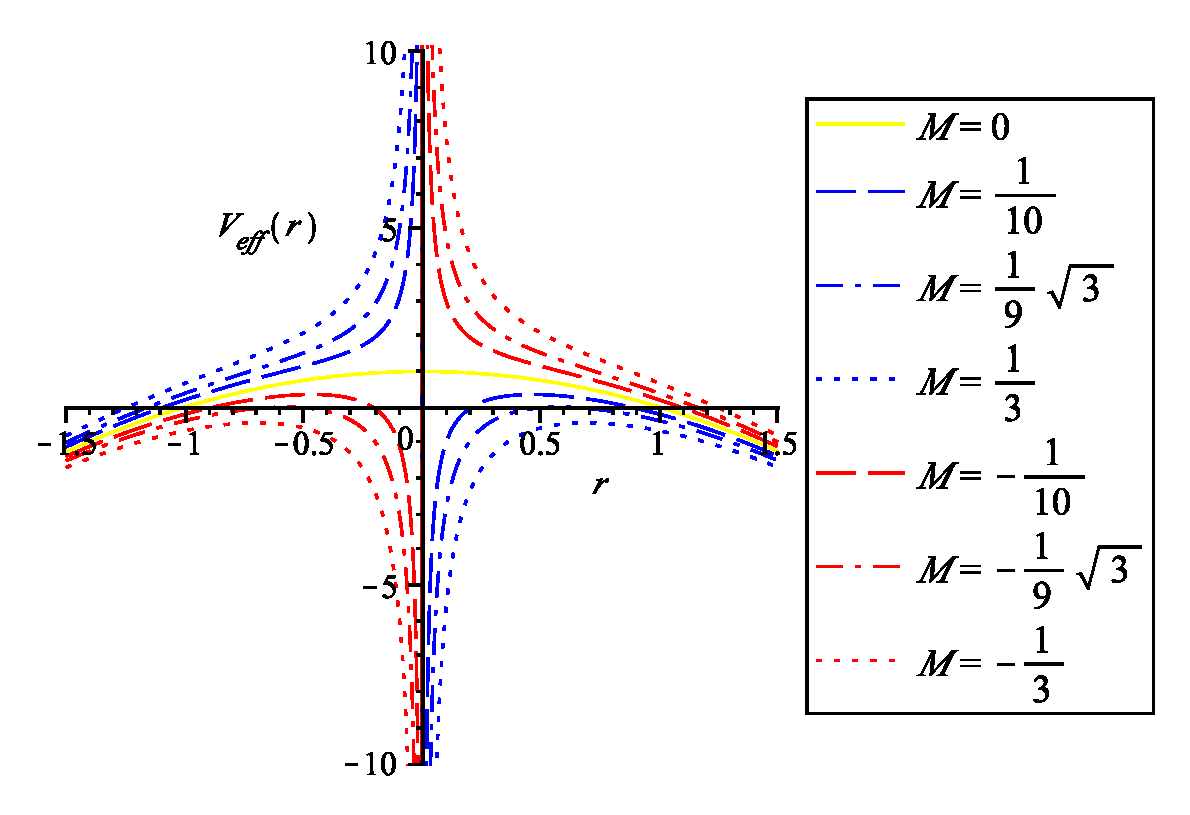
\includegraphics[width=6.5in]{SdS_Veff.eps}}
\caption[Effective potential of the SdS geometries.]{Scale-invariant effective potential curves for timelike geodesics with $J=0$, of SdS geometries with various values of $M$. Representative curves are plotted for the statical de~Sitter spacetime, and for under-critical, critical, and over-critical values of both positive and negative `mass'.}\label{SdS_Veff}
\end{figure}
In essence, the picture that now presents itself to us, according to Eq.~(\ref{V_eff}), which is plotted in Fig.~\ref{SdS_Veff} for representative values of the mass parameter, after setting $J=0$, is that of an initially homogeneous distribution of equal amounts of matter with positive and negative mass, with a natural tendency to dissociate into clusters of each species; all presumably with $|m|\ll1/\sqrt{\Lambda}$, so that the large-scale structure would remain homogeneous. However, to the inhabitants of any such cluster, the universe would appear to be filled only with clusters of the same form of matter, all separated by void regions of space---which would actually have been cleared of all visible matter by the dark anti-matter clustering there.

In order to describe rougly the local gravitational field surrounding a cluster which is large enough that its overall angular momentum should be negligible, consider that the mass density in its very near vicinity would be roughly equal to the value of its mass divided by the volume of the surrounding vacuum, as that would be cleared through this dissociation,---but that, as we've said above, the total density, on scales large enough that the mass distribution can be considered to be approximately homogeneous, and therefore sum to zero, must equal zero as well; therefore, the homogeneous clustering of matter surrounding any particular one, should result in an effective shell with mass roughly equal to negative that of the central cluster. Then, because the matter in that shell would actually repel the matter of which the central cluster is comprised, it should increase the effective gravitational attraction towards the centre---i.e., the existence of an effective negative mass shell surrounding a galaxy cluster, should affect its gravitational dynamics in much the same way as positive mass dark matter halos are thought to do---as the surrounding `voids', which would actually repel visible matter, would help to bind galaxy clusters more firmly than if they existed by themselves. As such, the large-scale appearance of this universe would be similar to that of our own.

And finally, it should not be difficult to imagine, that the increase in gravitational entropy, as the two forms of matter would cluster individually, could balance the decrease in thermodynamical entropy, according to which the universe would have been formed in a hot, homogeneous state. The constancy of this entropy is in fact demanded by the SdS geometry, as it must equal one-quarter of the horizon's `surface area' \cite{Padmanabhan2002c}; or, if the perceived mass of the universe were only slightly greater than the critical value, $|m_{univ}|\gtrsim1/\sqrt{\Lambda}$, the corresponding constant, total entropy would be $S_{univ}\gtrsim4\pi/\Lambda$.

\section{Modelling the Cosmology\label{sec_MC}}
We are finally set to determine the physical model that would correspond to observations within the cosmic rest-frame in this cosmology; and, in order to do this, we shall begin by transforming the statical line-element of the SdS geometry into the proper coordinate system in that frame. To this end, we shall begin from the equations of motion for timelike geodesics, Eqs.~(\ref{ttau_gamma}), (\ref{phitau_J}), and (\ref{rtau_J}). Now, Eq.~(\ref{phitau_J}) defines $J$ as a particle's specific angular momentum, which must be set to zero for all particles in the cosmic rest-frame, since $t$ is already defined as being parallel to their motion through the comoving universal 3-sphere given by Eq.~(\ref{dS_comoving_univ}). In order to properly interpret $\gamma$, however, we require some more care. 

It is helpful to momentarily restore dimensionality to the equations of motion, so that we may consider the Schwarzschild solution as a special case. With $J=0$, these reduce to only the two equations,
\begin{equation}
\frac{r-2M-\frac{\Lambda}{3}r^3}{r}\left(\frac{dt}{d\tau}\right)=\gamma,\label{ttau_gammaLambda}
\end{equation}
\begin{equation}
\left(\frac{dr}{d\tau}\right)^2=\gamma^2-\frac{r-2M-\frac{\Lambda}{3}r^3}{r};\label{rtau_Lambda}
\end{equation}
so that, when $\Lambda=0$, we can immediately identify the specific energy of a particle that would remain at rest at $r=\infty$ as the conserved quantity, $\gamma=dt/d\tau=1$. In fact, as shown in \S~25.3 of \cite{Misner1973}, the term `energy at infinity' applies generally to the term $\gamma{m_0}$, for any particle with rest mass $m_0$ anywhere in the Schwarzschild geometry, so that the value $\gamma=1$ need not be identified only with a particle that falls freely to or from rest at $r=\infty$, but actually, that its presence there need not ever be required---i.e., the term `energy at infinity' applies for any orbit at any $r$ in the Schwarzschild geometry, even if it cannot reach an observer at infinity who has the capability of measuring that quantity. 

But the value $\gamma=1$ does in fact have a more global interpretation in the SdS geometries, for which we find further evidence in noting that when $M$ is set to zero instead of $\Lambda$, it corresponds to a particle that would come to rest at the one inertial coordinate in the statical de~Sitter frame; i.e., if we require $dr/d\tau=0=d\phi/d\tau$ in Eqs.~(\ref{ttau_gamma}), (\ref{phitau_J}), and (\ref{rtau_J}), Eq.~(\ref{rtau_J}) reduces to $\gamma^2=1-r^2$, so that the specific energy of an inertial partile that would remain at $r=0$ is given by $\gamma^2=1$ as well. Conversely, if we set $\gamma^2=1$ to begin with, we find that the requirement for a particle to be spatially at rest, $dr/d\tau=0=d\phi/d\tau$, is satisfied only at $r=0$. In contrast to the pure Schwarzschild case, the value of $\gamma{m_0}$ in this geometry could therefore be referred to as a particle's `energy at the origin'.

But in general, it should be clear that the value $\gamma^2=1$ really corresponds to a particle that would be at rest in any SdS geometry where its gravitational potential vanishes identically---i.e., at $r=-\sqrt[3]{2M}$, where $V_{\mathrm{eff}}\equiv1$. And this fact can actually be used to define all particles with \textit{specific energy} $\gamma=1$ as the inhabitants of a preferred frame in these geometries, since (i.)~$t$ is always timelike at this coordinate, where the metric is actually identical to Minkowski space, so it is indeed appropriate to interpret $\gamma$ as the specific energy of a particle relative to that location, (ii.)~it must also be that any particle with $\gamma\neq1$, whose proper time would actually be different from $t$ there, according to Eq.~(\ref{ttau_gamma}), has some constant motion relative to a particle that would come to rest there, and (iii.)~according to the same point that was argued in \cite{Misner1973} for the Schwarzschild geometry, it really doesn't make a difference to this interpretation if such a particle cannot physically come to this point, which is indeed only possible outside a negative SdS mass. Therefore, we interpret $\gamma$ as a particle's `specific energy in the cosmic rest-frame' of any SdS geometry---and, e.g., set $\gamma=1$ in order to describe the trajectory of an inertial particle that is `at rest' in the cosmic rest-frame of an over-critical SdS universe.

Before proceeding with the relevant coordinate transformation to the line-element that describes this frame, let us first consider an example which further illustrates the meaning of this point. As noted already in \S~\ref{sec_TSC} (cf.~Eq.~(\ref{r_e})), a test-particle can remain at rest at $r=M^{1/3}$, in the largest possible `circular orbit' around an SdS mass with mass parameter $M$. This radius is found by solving $dV_{\mathrm{eff}}(r)/dr=0$ for $r$, after setting $J=0$ as the lowest value of angular momentum that may be allowed for such an orbit. Now, the total specific energy of such a particle is given by $\gamma^2=1-3M^{2/3}$, according to Eq.~(\ref{rtau_J}); however, rather than interpreting this as corresponding to the particle's potential energy as it remains at rest in space in the gravitational field, we interpret it as corresponding to the difference between its specific energy in the cosmic rest-frame and a kinetic energy term due to the fact that it is not `at rest' in \textit{that} frame. This simply illustrates the equivalence of gravitational mass and inertial mass, that is described by general relativity theory.

We shall now determine how, in general, the SdS geometries would be perceived in the frame of an observer with $\gamma=1$, by finding the coordinate system that describes the bundle of timelike geodesics which move through $t$ and $r$ all at the same rate, $\tau$, and occupy constant positions in `space'. The expressions for the proper velocities through $t$ and $r$ of these comoving geodesics can immediately be written from Eqs.~(\ref{ttau_gamma}) and (\ref{rtau_J}) with $\gamma=1$ and $J=0$:
\begin{equation}
\partial_{\tau}{t}\equiv\frac{\partial{t}}{\partial\tau}=\frac{r}{r-2M-r^3},\label{tdot}
\end{equation}
\begin{equation}
(\partial_{\tau}r)^2\equiv\left(\frac{\partial{r}}{\partial\tau}\right)^2=\frac{2M+r^3}{r}.\label{rdot}
\end{equation} 

The solution of Eq.~(\ref{rdot}) may be expressed in closed-form, by using the standard integral, $\int\left(u^2+a\right)^{-1/2}du=\ln\left(u+\sqrt{u^2+a}\right)$, after substitution of a new variable, $u^2=2M+r^3$. Taking the positive root of Eq.~(\ref{rdot}) for outgoing geodesics, we have,
\begin{equation}
\tau=\int^{r(\tau)}_{r(0)}\sqrt{\frac{r}{2M+r^3}}dr=\left.\frac{2}{3}\ln\left(\sqrt{2M+r^3}+r^{3/2}\right)\right|^{r(\tau)}_{r(0)},\label{t_int}
\end{equation}
where the lower limit on the proper time has been arbitrarily set to zero. Thus, in this frame we can express the statical coordinate $r$ of the SdS geometry as a function of each observer's proper time and a synchronous spatial coordinate, $r(0)$, which may be arbitrarily rescaled without significantly altering the description.

Then, as long as $M$ is nonzero, a convenient set of coordinates from which to proceed results from rescaling this coordinate as,\footnote{Note that this transformation is not valid when $M=0$, which we are anyhow not interested in. An equivalent transformation in that case is found by setting $r(0)\equiv{e}^{f(\xi)}$, whence $r(\tau,\xi)=e^{\tau+f(\xi)}$, and Eqs.~(\ref{g_chit}), (\ref{g_tt}), and (\ref{g_chichi}), below, yield the line-element, $ds^2=-d\tau^2+r^2\left(d\xi^2+d\theta^2+\sin^2\theta{d\phi^2}\right)$.} 
\begin{equation}
r(0)\equiv(2M)^{1/3}\sinh^{2/3}\left(\frac{3}{2}f(\xi)\right) ;~M\neq0, \label{r(0)}
\end{equation}
from which we find, after some rearranging,\footnote{Note that the two identities, $e^x=\sinh(x)+\cosh(x)$ and $\mathrm{arsinh}(x)=\ln\left(x+\sqrt{x^2+1}\right)$, are useful here. Eq.~(\ref{r(tau,xi)}), along with our eventual line-element, Eq.~(\ref{SdS_proper}), was originally found by Lema\^{i}tre \cite{Lemaitre1949}, although his solution to Eq.~(\ref{rdot}) (with dimensionality restored),
\[r=(6M/\Lambda)^{1/3}\sinh^{2/3}\left[3\sqrt{\Lambda}(t-t_0)/2\right],\]
is too large in its argument by a factor of $\sqrt{3}$.}
\begin{equation}
r(\tau,\xi)=(2M)^{1/3}\sinh^{2/3}\left(\frac{3}{2}[\tau+f(\xi)]\right),\label{r(tau,xi)}
\end{equation}
which immediately shows the usefulness of expressing the arbitrary coordinate $\xi$ in the form written in Eq.~(\ref{r(0)}), because it allows Eq.~(\ref{t_int}) to be solved explicitly for $r(\tau,\xi)$. Therefore, without loss of generality, we define a new coordinate $\chi\equiv{f(\xi)}$, so that $-\tau\leq\chi\leq\infty$. This has no effect on the eventual form of the metric we will derive, due to the chain rule, but allows for a neater calculation. As such, we immediately have the useful result,
\begin{equation}
\partial_{\chi}r\equiv\frac{\partial{r}}{\partial\chi}=\partial_{\tau}r=\sqrt{\frac{2M+r^3}{r}}.\label{rprime}
\end{equation}

The transformation, $t(\tau,\chi)$, may then be calculated from
\begin{equation}
\frac{dt}{dr}=\frac{\partial_{\tau}t}{\partial_{\tau}r}=\frac{r}{r-2M-r^3}\sqrt{\frac{r}{2M+r^3}};
\end{equation}
furthermore, to solve for $t(\tau,\chi)$, we can gauge the lower limits of the integrals over $t$ and $r$, at $\tau=0$, by requiring that their difference, defined by 
\begin{equation}
t(\tau,\chi)=\int^{r(\tau,\chi)}\frac{r}{r-2M-r^3}\sqrt{\frac{r}{2M+r^3}}dr-F(\chi),\label{t(tau,chi)}
\end{equation}
sets 
\begin{equation}
g_{\chi\tau}=g_{tt}\partial_{\tau}t\partial_{\chi}t+g_{rr}\partial_{\tau}r\partial_{\chi}r=0.\label{g_chit}
\end{equation} 
This calculation is straightforward:
\begin{eqnarray}
0\!\!\!&=&\!\!\!-\frac{r}{r-2M-r^3}+\partial_{\chi}F(\chi)+\frac{r}{r-2M-r^3}\frac{2M+r^3}{r}\\
\!\!\!&=&\!\!\!\partial_{\chi}F(\chi)-1,
\end{eqnarray}
so that $F(\chi)=\chi$.

Now, it is a simple matter to work out the remaining metric components as follows: our chosen reference frame immediately requires 
\begin{equation}
g_{\tau\tau}=g_{tt}(\partial_{\tau}t)^2+g_{rr}(\partial_{\tau}r)^2=-1,\label{g_tt}
\end{equation} 
according to the Lagrangian, Eq.~(\ref{L_timelike}), with $\partial\phi/\partial\tau=0$; and by direct calculation, we find
\begin{eqnarray}
g_{\chi\chi}\!\!\!&=&\!\!\!g_{tt}(\partial_{\chi}t)^2+g_{rr}(\partial_{\chi}r)^2\\
\!\!\!&=&\!\!\!-\frac{r-2M-r^3}{r}\left(\frac{2M+r^3}{r-2M-r^3}\right)^{2}+\frac{r}{r-2M-r^3}\frac{2M+r^3}{r}\\
\!\!\!&=&\!\!\!(\partial_{\chi}r)^2.\label{g_chichi}
\end{eqnarray} 
But this result is independent of the definition of $\chi$, as explained above; for if we had followed through with the more general coordinate $\xi$, we would have found the metric to transform as $g_{\xi\xi}=g_{\chi\chi}(d\chi/d\xi)^2=(\partial_{\xi}r)^2$, the other components remaining the same. Therefore, the SdS metric in the proper frame of an observer who is cosmically `at rest', in which the spatial coordinates are required, according to an appropriate definition of $F(\chi)$, to be orthogonal to $\tau$,\footnote{Note that $\theta$ and $\phi$ were already orthogonal to $\tau$.} can generally be written,
\begin{equation}
ds^2=-d\tau^2+\left(\partial_{\chi}r\right)^2d\chi^2+r^2\left(d\theta^2+\sin^2\theta{d\phi}^2\right).\label{SdS_proper}
\end{equation}

Thus, we have proven Lema\^{i}tre's result from 1949 \cite{Lemaitre1949},---that spaces with $d\tau=0$ are Euclidean, with line-element,
\begin{equation}
d\sigma^2=dr^2+r^2\left(d\theta^2+\sin^2\theta{d\phi}^2\right).
\end{equation}
Lema\^{i}tre concluded from his calculation, that the `geometry is Euclidean on the expanding set of particles which are ejected from the point singularity at the origin', which is represented in this frame by the line $\chi=-\tau$; but he did not proceed to develop a cosmology directly from this result. Instead, for the universe as a whole, he cast the geometry aside, writing that, in the case of such a singularity, `the particles continuously ejected have no physical reality; they are just mathematical devices introduced in order to define the coordinates and the corresponding partition of space and time', and proceeded with the development of a FLRW cosmological model, eventually applying this result in a statement, that `in order that spherical symmetry should exist around any point, we must particularize the results found for spherical symmetry, so that the three spatial coordinates $\theta$, $\phi$, and $\chi$ would appear in the expression $d\sigma$ only'. This, he accomplished by redefining $r$ as a separable function of the coordinates $\chi$ and $\tau$, which is impossible in the SdS geometry, according to Eq.~(\ref{r(tau,xi)}), since, aside from the trivial case ($x$ or $y\equiv0$), the hyperbolic sine function cannot be written $\sinh(x+y)=A(x)B(y)$. As such, his new $d\sigma$---the RW spatial line element---would bear no relation to the original geometry from which it had been calculated.

Essentially what he did was to interpret the synchronous set of events in this spacetime as the comoving universe---which is false, as one should understand according to the discussion of Chapter~\ref{chap_DIRT}; for, by the definition that was finally given in Eq.~(\ref{sphersymm_r}), the dynamic universe described by the over-critical SdS spacetime should actually be comoving along $r$.

It is interesting, and clarifies the physical meaning of this result, to recheck our calculation by beginning with the expression we've found for the cosmic radius, Eq.~(\ref{r(tau,xi)}). According to this expression, spaces of a given radius must have the same value, $\bar\tau\equiv\tau+\chi$; and the set of comoving inertial observers described by Eq.~(\ref{SdS_proper}), who each remain at constant $\chi$, and whose clocks all tick at the same rate $\tau$, must coexist dynamically on the causal hypersurface $\tau=\bar\tau-\chi$, rotated an angle $\pi/4$ from the $\tau$-axis, in the $(\tau,\chi)$-plane; thus, $\bar\tau$ is the cosmic time of the bundle of geodesics defining the cosmic rest frame. And this fact may be used to rewrite the statical and proper line-elements for the SdS geometry, using notation which is meaningful to observers who are cosmically `at rest', according to the total derivative of $r$ with respect to the cosmic time,
\begin{equation}
\frac{dr}{d\bar\tau}=\left(2M\right)^{1/3}\frac{\cosh\left(3\bar\tau/2\right)}{\sinh^{1/3}\left(3\bar\tau/2\right)}=\sqrt{\frac{2M+r^3}{r}},\label{drdbartau}
\end{equation}
after noting, from Eq.~(\ref{t(tau,chi)}), the corresponding transformation of the coordinate $t$,
\begin{eqnarray}
dt\!\!\!&=&\!\!\!\nonumber{\frac{r}{r-2M-r^3}\sqrt{\frac{r}{2M+r^3}}dr-d\chi},\\
\!\!\!&=&\!\!\!-\left[\left(\frac{dr}{d\bar\tau}\right)^2-1\right]^{-1}(d\tau+d\chi)-d\chi.
\end{eqnarray}
These may be substituted directly into the statical SdS metric, Eq.~(\ref{SdS_statical_pure}). Then the statical and proper line-elements are, respectively,
\begin{eqnarray}
ds^2\!\!\!&=&\!\!\!-\left[\left(\frac{dr}{d\bar\tau}\right)^2-1\right]^{-1}dr^2+\left[\left(\frac{dr}{d\bar\tau}\right)^2-1\right]dt^2+r^2\left(d\theta^2+\sin^2\theta{d\phi^2}\right),\label{SdS_statical_bartau}\\
\!\!\!&=&\!\!\!-d\tau^2+\left(\frac{dr}{d\bar\tau}\right)^2d\chi^2+r^2\left(d\theta^2+\sin^2\theta{d\phi^2}\right),\label{SdS_proper_bartau}
\end{eqnarray}
from which it is obvious that the critical condition for $r>0$ to be timelike, $M>1/\sqrt{27}$, must be equivalent to the requirement, $(dr/d\bar\tau)^2>1$. This may be confirmed using Eq.~(\ref{drdbartau}), from which we find that $dr/d\bar\tau$ has a minimum at the inflection point, $3\bar\tau_{accel}=\ln\left(2+\sqrt{3}\right)=2\,\mathrm{arsinh}\left(1/\sqrt{2}\right)$, of $r(\bar\tau)$, at which particles begin to accelerate away from $r=0$. Substituting this value back into Eq.~(\ref{drdbartau}), we find, 
\begin{equation}
{\left.\frac{dr}{d\bar\tau}\right|}_{\sinh\left(3\bar\tau_{accel}/2\right)=1/\sqrt{2}}=\left(2M\right)^{1/3}\frac{\sqrt{3/2}}{2^{-1/6}}=\sqrt{3}M^{1/3};\label{rdot_crit}
\end{equation}
so that, indeed, $(dr/d\bar\tau)^2>1$ for all $\bar\tau\Leftrightarrow{M}>1/\sqrt{27}$.

What we would now like to understand, is how such a universe would appear to an observer in the cosmic rest-frame, who observes light which has causally propagated \textit{through} the void \textit{within} the non-synchronous universe; so, in order to illustrate this situation, various null-lines of constant $\theta$ and $\phi$,
\begin{equation}
\frac{d\tau}{d\chi}=\pm\frac{dr}{d\bar\tau},
\end{equation}
have been plotted in Fig.~\ref{over-critSdS_Null}, in the $(\tau,\chi)$-plane of the $M=1/2~(>1/\sqrt{27})$ SdS geometry, alongside the corresponding section of the de~Sitter sphere, from Fig.~\ref{fig: dS_comoving_univ}.
\begin{figure}[t!]
\centerline{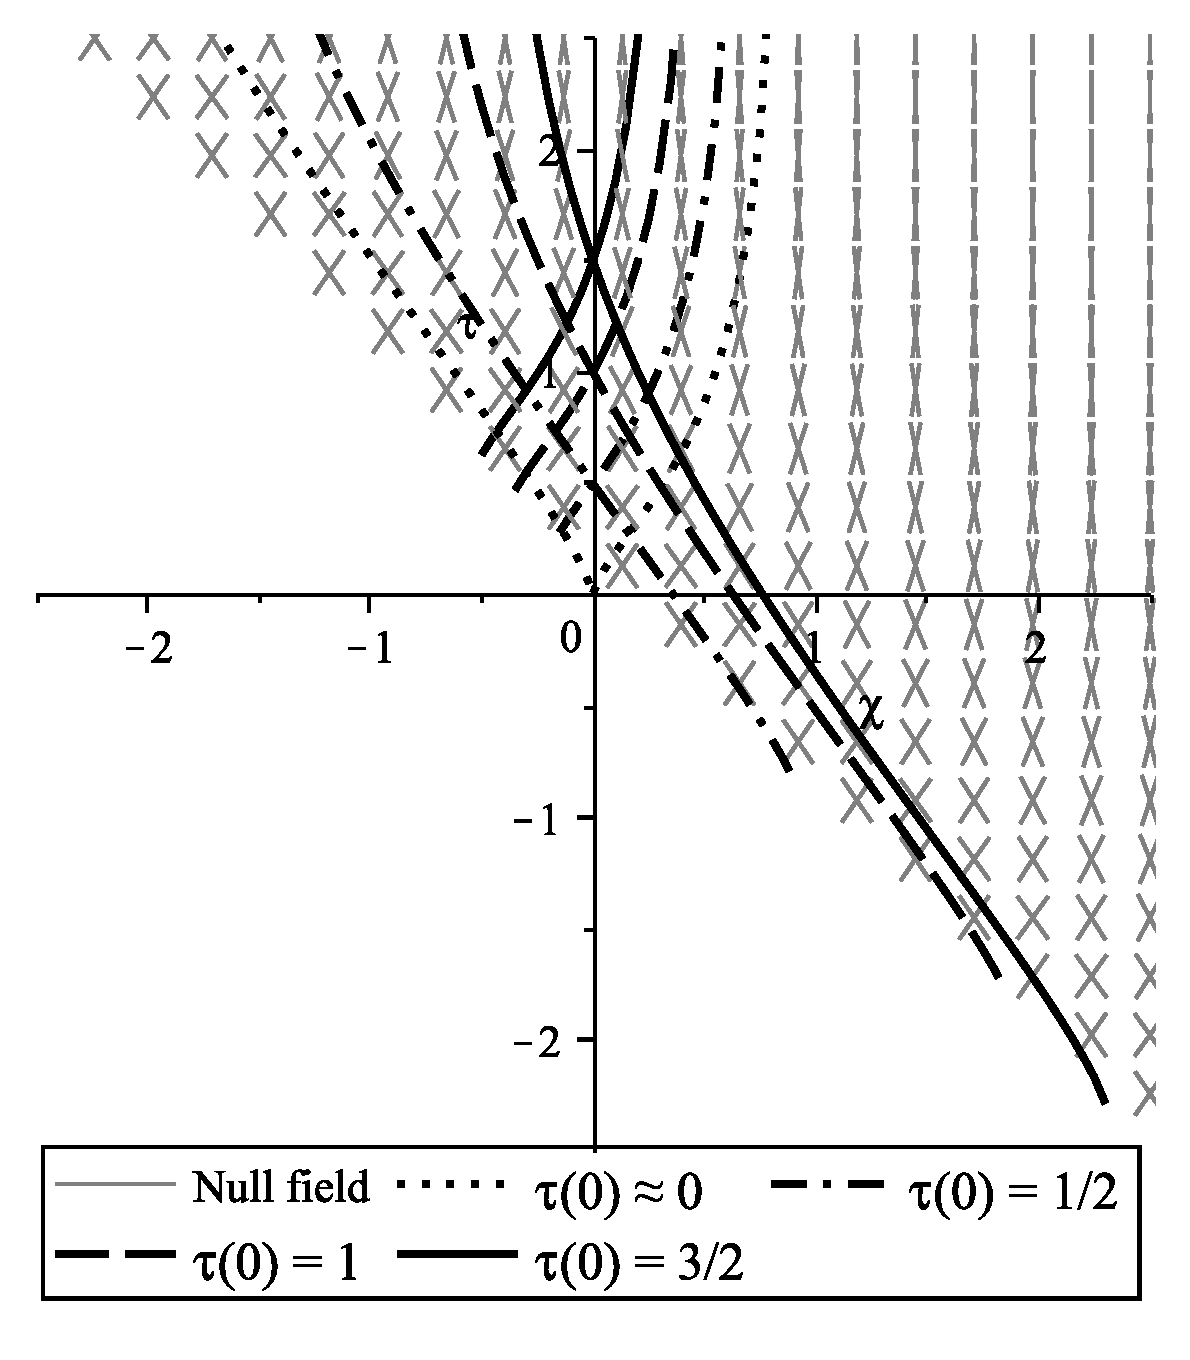
\includegraphics[width=3.05in]{over-critSdS_Null.eps}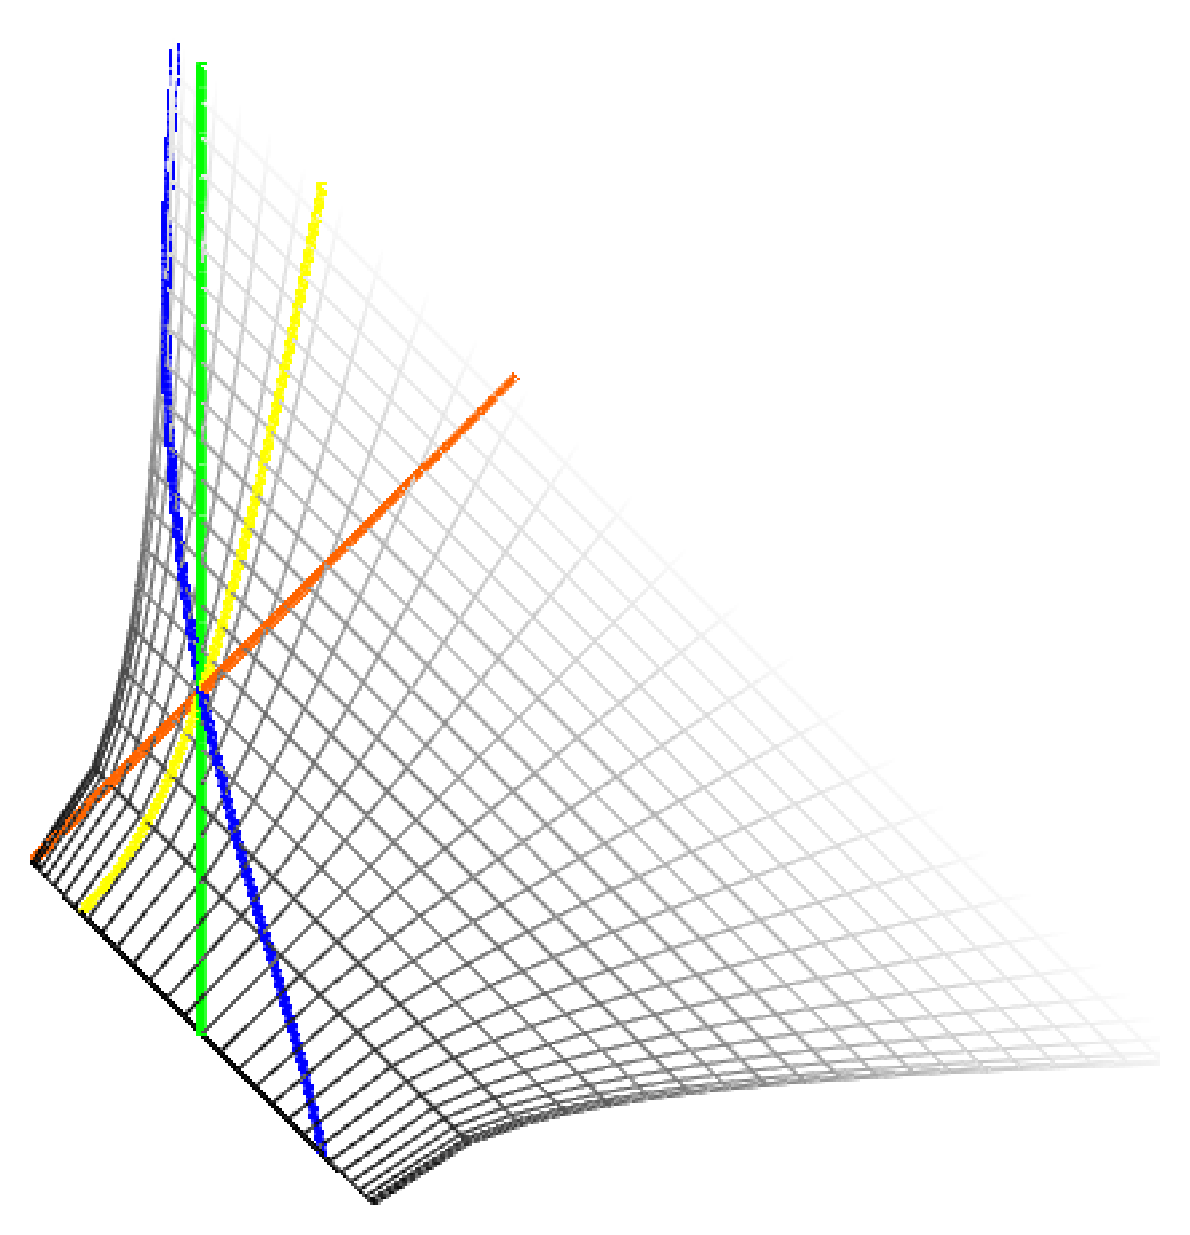
\includegraphics[width=3.45in]{dS_SdS_sim.eps}}
\caption[Null geodesics in the $(\tau,\chi)$-plane of an `over-critical' SdS geometry.]{Null geodesics in the $(\tau,\chi)$-plane of the SdS geometry with $M=1/2>1/\sqrt{27}$ (left), plotted alongside the corresponding section of the de~Sitter sphere (right; see Fig.~\ref{fig: dS_comoving_univ}). A universe must evolve along one increasing radius, with cosmic time $\bar\tau=\tau+\chi$, comoving at a forty-five degree angle from the $\tau$-axis. By design, particles at-rest in the cosmic rest-frame follow flat null-lines through de~Sitter space, with `simultaneous space' at any particular value of proper time described by the oppositely-directed null-line passing through that event.}\label{over-critSdS_Null}
\end{figure}

With this diagram, it can be easily pictured how light approaching an observer from positive or negative $\chi$ originates from prior $\bar\tau$, and is emitted, in either direction, towards increasing $\bar\tau$, even though, at any $\tau$, every observer perceives simultaneous space as the flat slice of spacetime ranging from $\bar\tau=0$ to $\bar\tau=\infty$, with the `big bang' singularity at $\chi=-\tau$ (cf.~Lema\^{i}tre's interpretation of particles continuously ejected from the point singularity at the origin). The associated graph of de~Sitter space, in which one of the flat null-lines has been oriented vertically, so that it would correspond to the $\tau$-axis of the particle at $\chi=0$, shows that the $\tau$- and $\chi$-coordinates should be the collections of oppositely directed (flat) null-lines on the de~Sitter sphere, which run parallel to each other in the coordinate system of Eq.~(\ref{SdS_proper})---i.e., the coordinate system we use to describe spacetime in the cosmic rest-frame of the `over-critical SdS universe' takes the flat null-lines of the de~Sitter sphere and lays them out orthogonally on a plane;---and the association, of null-lines in that coordinate system, to the `photons' defined in our theory (which are represented in Fig.~\ref{over-critSdS_Null} by blue and yellow world-lines) is likewise apparent. As well, it is clear that massive particles should evolve between those null-lines in either picture, and that the world-lines of particles with `negative mass'---i.e., those which move in the opposite direction through the comoving universal 3-sphere---should indeed be spacelike, as we effectively defined from the outset (i.e., at the end of \S~\ref{sec_RPT}). Thus, e.g., the world-line of a particle that follows an oppositely directed null-line on the de~Sitter sphere, such as the centres of mass of `dark anti-matter clusters' postulated to exist in \S~\ref{sec_DPM}, would be described as occurring all at an instant in the $(\tau,\chi)$-frame.

But this ideal spacetime description, according to which some particles or massive clusters would run their entire course of existence in an instant, and others could even be said to move backwards in time, cannot actually be an accurate description of the cosmological evolution that would be observed, since the comoving universe does not actually exist synchronously with any such observer, and when cosmological measurements happen to be made, the observer must still see the real causal evolution that has taken place in \textit{cosmic} time. 

So we must now put together the pieces of our description, in order to say precisely how physical observables should be modelled in this frame. To begin with, we note that the cosmological redshift of light emitted from anywhere in the homogeneous universe at some earlier cosmic time, $\bar\tau_{e}$, and observed presently, at $\bar\tau_0$, must be given---either according to the real physical expansion of the universe, or else the perceived difference in effective potential---by 
\begin{equation}
1+z=\frac{r(\bar\tau_0)}{r(\bar\tau_e)}.\label{z_SdS}
\end{equation}
Also, because cosmic rest-frame observers travel along null-lines of the de~Sitter sphere, all propagating in the same direction and fanning out as cosmic time increases, the perceived expansion based on a homogeneous distribution of galaxies travelling along those fundamental worldlines, must still be isotropic from the relative perspectives of such observers. Finally, we have the two relevant\footnote{Actually, the flatness of synchronous slices in the fundamental rest-frame is probably not relevant at all, since the curvature of RW space only enters into cosmological observations through the scale-factor, and we anyhow have the result that $r(\bar\tau)$ scales precisely as the \textit{flat} $\Lambda$CDM scale-factor, in a universe that essentially \textit{is}, and must also \textit{appear} isotropic to all observers in the fundamental rest-frame; i.e., because through standard FLRW theory, all we really measure through cosmological observations is the form of $a$ as a function of $t$, which must satisfy Eqs.~(\ref{Friedmann}), (\ref{Friedmann2}), and basic assumptions about the large-scale perfect fluidity of the universe; and we have already derived such a scale-factor in a very different way, as a specific function which is equivalent to the very specific such model in which $K=0$, $p=0$, and $\Lambda\neq0$.} frame-specific aspects of perception: that the simultaneous slices of spacetime in the observer's past light-cone are flat, and that $r$ is given as a specific function of the proper time of any such observer, so that the line-element that would be appropriate for modelling physical observables within this cosmology must be the one corresponding to a flat RW expansion, with $K=0$ in Eq.~(\ref{RW}), and,
\begin{equation}
a(\bar\tau)\equiv{r}(\bar\tau)=(2M)^{1/3}\sinh^{2/3}\left(3\bar\tau/2\right);\label{a_SdS_pure}
\end{equation}
or, restoring units $(a\mapsto\sqrt{\Lambda/3}a'=a)$,
\begin{equation}
a(\bar\tau)=\left(\frac{6M}{\Lambda}\right)^{1/3}\sinh^{2/3}\left(\frac{3}{2}\sqrt{\frac{\Lambda}{3}}\bar\tau\right).\label{a_SdS}
\end{equation}

It is not difficult to derive Eq.~(\ref{a_SdS}) as the solution to Friedman's equations, Eqs.~(\ref{Friedmann}) and (\ref{Friedmann2}), for a flat $\Lambda$CDM universe with $p=K=0$, by direct integration. However, this is unnecessary because the same can be proven simply by showing that $\dot{a}/a$, as calculated directly from Eq.~(\ref{a_SdS}), is equal to the flat $\Lambda$CDM \textit{Hubble parameter}, since the requirement that $a(\bar\tau=0)=0$ is already satisfied. In doing so, we'll find an interesting connection to the SdS mass parameter, $M$.

To begin as usual, note that compatibility of Friedman's equations requires
\begin{equation}
\dot{\rho}=-3(\rho+p)\frac{\dot{a}}{a},
\end{equation}
which may be used in place of Eq.~(\ref{Friedmann2}), so that a FLRW universe containing only nonrelativistic matter, with $p\ll\rho\equiv\rho_m$, satisfies
\begin{equation}
\rho_m{a^3}=\rho_{m,0}{a_0}^3=const.,\label{varrho}
\end{equation}
where the subscript 0 denotes evaluation at the present time, $\bar\tau_0$. Then, with $K=0$ and general $\Lambda$, Eq.~(\ref{Friedmann}) may be rewritten,
\begin{equation}
H\equiv\frac{\dot{a}}{a}=\sqrt{\frac{\Lambda}{3}+\frac{\kappa\rho_m{a}^3}{3a^3}},
\end{equation}
where $H$ is the Hubble parameter. This is the flat $\Lambda$CDM Friedman equation, expressing $\dot{a}$ as a function of $a$ only, which has been quite precisely constrained through observations of the CMB, SNe Ia, and other phenomena, this past decade.

But, noting that $\coth(\mathrm{arsinh}\,(x))=\sqrt{1+x^{-2}}$, this same result follows immediately when we write the Hubble parameter according to Eq.~(\ref{a_SdS}); i.e., because then
\begin{eqnarray}
\frac{\dot{a}}{a}\!\!\!&=&\!\!\!\nonumber{\sqrt{\frac{\Lambda}{3}}\coth\left(\frac{3}{2}\sqrt{\frac{\Lambda}{3}}\bar\tau\right),}\\
\!\!\!&=&\!\!\!\sqrt{\frac{\Lambda}{3}+\frac{2M}{a^3}},\label{Hubble_param}
\end{eqnarray}
so that, with $\kappa\equiv8\pi$, we can immediately identify
\begin{equation}
M=\frac{4\pi}{3}a^3\rho_m\label{M_density}
\end{equation}
as the apparent constant mass per unit comoving volume in the perceived flat $\Lambda$CDM universe. This quantity cannot be determined through redshift measurements though, because those correspond to the ratio, $a_0/a_e$, between the present scale-factor and its value at the epoch which is presently being observed, and $M$ vanishes from that quantity. More explicitly, the luminosity distance of an object with redshift $z$ may be calculated from $(u\equiv{{a_0/a})$
\begin{equation}
d_{L}=(1+z)\int_1^{1+z}\frac{du}{H(u)}=(1+z)\int_1^{1+z}\frac{du}{\sqrt{\frac{\Lambda}{3}+\left({H_0^2-\frac{\Lambda}{3}}\right)u^3}},
\end{equation}
so that $\Lambda$ and the \textit{Hubble constant}, $H_0$, can, e.g., be determined by modelling the apparent magnitude ($m_{\textrm{mag}}$) distribution of a sample of \textit{standard candles} (all with the same absolute magnitude, $M_{\textrm{mag}}$, such as SNe Ia) according to the distance modulus equation,
\begin{equation}
m_{\textrm{mag}}-M_{\textrm{mag}}=5\log_{10}\left(\frac{d_L}{10~\mathrm{pc}}\right).
\end{equation}
But then, according to Eqs.~(\ref{Hubble_param}) and (\ref{M_density}), only values such as $\bar\tau_0$, $M/{a_0}^3$, and $\rho_{m,0}$ can be calculated subsequently. Even so, we can say (for what it's worth) that $M$ has to be greater than the limit set by the over-critical condition, $\sqrt{\Lambda/3}M>1/\sqrt{27}$; or, using $\Lambda\sim10^{-52}~\mathrm{m}^{-2}$, $M>1/(3\sqrt{\Lambda})\sim5\times10^{52}$~kg.

\section{Cosmic Black Holes and an Omniverse\label{sec_CBHO}}
Let us consider finally, how such a universe as the one that has now been described should be created through the eventual gravitational collapse of a system of galaxies that existed in a prior one. There is in fact little that needs to be said in order to complete this picture, since the physical scenario that is left for us to state should already be obvious to one who has followed the prior theoretical development to this point. So, while keeping in mind some of the main aspects of the theory---viz., the fact that the ideal evolution of our universe is given by the SdS line-element, which similarly describes a spacetime that is locally dominated by a spherical mass, and that the universe should fully run its course only on the `expanding half' of de~Sitter space---we shall revisit the problem of gravitational collapse.

%For, to anyone who has studied that prior development, the few immediate implications that may be deduced from that theory regarding a connection between the causal process of gravitational collapse and the creation of universes in a greater omniverse, should be completely obvious; whereas, to one who does not understand the theory that has been presented, this conclusion shall seem entirely fantastical. The reason I say this, is that the justification for the conclusions that are drawn below, will seem incomplete to anyone who does not fully appreciate the many crucial points in the analytical theory presented above which differ significantly from commonly held beliefs,---not the least of which being the general deviation from the current epistemological paradigm in physics, which would deny rationalisation its place next to practical observation and mathematical formulation, when developing new theories to account for the empirical facts. For, as I have tried to argue from the outset, the aim here has never been---as indeed it never has been for those who have sought an accurate understanding of things---to work out only an empirical model that could be used to accurately describe the phenomena, but to work out a practical \textit{and} rational theory that would describe the phenomena \textit{and} explain why they should be as they appear. For twentieth century cosmology has made it abundantly clear, that a non-rational theory shall always be wrought with significant problems which it cannot explain, whereas rational axiomatic reduction of our physical description of Nature has always led to a clearer and more coherent idea of what It is, resolving such problems as abound our currently beloved description.

According to our theory, local expansion dynamics should really be occurring in roughly the manner examined by Lema\^{i}tre \cite{Lemaitre1933,Lemaitre1997,Lemaitre1934,Lemaitre1949,Lemaitre1952,Lemaitre1958} (or, e.g., de~Sitter \cite{deSitter1933a}, Eddington \cite{Eddington1933}, or Pirani \cite{Pirani1954}), which was briefly discussed in \S~\ref{sec_TSC}. Therefore, roughly speaking, as the Universe evolves, every galaxy or cluster of galaxies with no net angular momentum, which is denser than the limit set by Eq.~(\ref{r_e}), will remain gravitationally bound in the face of cosmic expansion that is driven by $\Lambda$. According to the standard theory of galactic dynamics (e.g., see \cite{Schweizer1986,Krauss2000}), every such localised pocket of matter shall evolve, through the interactions of its constituent parts, into a single giant elliptical galaxy, again with roughly no net angular momentum or charge; which, through subsequent relaxing processes, shall, according to the spacetime dynamics of gravitational collapse described above, inevitably collapse to a critically dense SdS configuration, asymptotically falling towards its `event horizon' as everything else in the Universe recedes exponentially.

According to this picture, even the collapse of a single star is not to be thought of as having a very close connection to the final state---for although the collapsing star will appear to `freeze' at its Schwarzschild radius and remain there for a very long time, it will not remain in that solitary state forever, but shall eventually come in close contact with other bodies, and dynamically interact with them in many possible ways; i.e., although a particle on the star's surface could be thought to reach the star's Schwarzschild radius in a small interval of proper time, it cannot reach any such horizon before every eventual interaction of the frozen star has taken place and the end result of all those interactions has come to the final one just described, so that the horizon it will come to will be very different from the one it initially began falling towards.

Now we must consider the final description of this collapse. The possibilities that have anything to do with the traditional conception, in which the central regions should cross an inner horizon first, and the inner timelike interval of $r$ should grow until all of the collapsing material has entered the black hole, are completely denied by this causally coherent description. For in fact, even if we attempt to reconcile this idea with the fact that interior particles cannot fall through inner horizons before the outer particles do, by suggesting that every particle should reach a limiting inner radius `at once', so that there is a sort of `instant'\footnote{According to the language that was developed in \S~\ref{sec_OJGKD}, this would be an instant in the five-dimensional ideality (if such could be given when causal coherence is not assumed \textit{a priori}) of the four-dimensions of reality.} at which all particles that comprised the former `frozen star' should now be distributed \textit{throughout} the interval of now-timelike $r$, we still have a violation of causal coherence, as these particles should no longer inhabit one universe.

In fact, the possibility that remains, is that the particles, which all inhabited the same universe with local measure of cosmic time described by $t$ at $r=\sqrt[3]{-2M}$ before the horizon, must \textit{universally} collapse, with subsequent cosmic evolution occurring radially. 

The picture that this brings to mind is an unfortunate three-dimensional one, involving a 2-sphere that is somehow created in space just prior to collapse, which subsequently contracts as it evolves towards $r=0$---and that is incorrect. But rather than trying to talk about all of the reasons that this should be incorrect, according to the four-dimensional theory of relativistic dynamics, without the clarity that would be afforded by an analytical solution, it seems best to simply end this discussion with a conjecture: that the product of this collapse is a 3-sphere in de~Sitter space, similar to our universe, which may also be described globally by the \textit{over}-critical SdS line-element, with velocities randomly oriented in all directions in that collapsing 3-sphere, so that our previous assumptions about the fundamental cosmic rest-frames of positive and negative mass particles should similarly apply; i.e., so that, from the collapse of a cluster with positive \textit{or} negative \textit{under}-critical SdS mass, which should reach its horizon at infinite cosmic time, a collapsing \textit{over}-critical SdS universe should emerge with a perfectly random distribution of particle velocities. This universe should then collapse to a finite radius in de~Sitter space, or else all the way to the `singularity' at $r=0$ in the over-critical SdS geometry pertaining to the fundamental rest-frame of massive particles, before subsequently expanding in the manner that has been described.

Such an origin for our universe would finally answer the problem of the cause of cosmic time, that needed to be left unanswered at the end of \S~\ref{sec_RPT}; for although the Lorentzian signature of de~Sitter space and the homogeneity of the actual universe described by Eq.~(\ref{dS_comoving_univ}) had indicated that this was a good possibility to explore, the description that is offered by the mathematics still does not indicate what would cause the universe to be this moving 3-sphere. However, if such a universe could thus be described as the direct result of a process which has been confirmed to take place in our Universe---viz., of the inevitable final stage of gravitational collapse of massive bodies,---then we could indeed attribute this as a prior natural cause of the cosmic geometry and time prescribed in our theory, which corresponds well with cosmological observations.  

Then we could infer the existence of a great number of universes similar to our own---each one the product of gravitational collapse in a progenitor universe that became a multiverse when its infinite course had ended. The logical extrapolation of this is to an omniverse: an infinite pattern of such past and future universes. Then, as the process of beginning in the omniverse should not be singular, it is reasonable to suggest that each universe should retain some information from its progenitor cluster, as similarly considered elsewhere \cite{Tolman1931,Misner1973,Smolin1997}.